\documentclass{beamer}
\usepackage[utf8]{inputenc}

\usetheme{Madrid}
\usecolortheme{default}
\usepackage{amsmath,amssymb,amsfonts,amsthm}
\usepackage{txfonts}
\usepackage{tkz-euclide}
\usepackage{listings}
\usepackage{adjustbox}
\usepackage{array}
\usepackage{tabularx}
\usepackage{gvv}
\usepackage{lmodern}
\usepackage{circuitikz}
\usepackage{tikz}
\usepackage{graphicx}
\usepackage{multicol}

\setbeamertemplate{page number in head/foot}[totalframenumber]

\usepackage{tcolorbox}
\tcbuselibrary{minted,breakable,xparse,skins}



\definecolor{bg}{gray}{0.95}
\DeclareTCBListing{mintedbox}{O{}m!O{}}{%
  breakable=true,
  listing engine=minted,
  listing only,
  minted language=#2,
  minted style=default,
  minted options={%
    linenos,
    gobble=0,
    breaklines=true,
    breakafter=,,
    fontsize=\small,
    numbersep=8pt,
    #1},
  boxsep=0pt,
  left skip=0pt,
  right skip=0pt,
  left=25pt,
  right=0pt,
  top=3pt,
  bottom=3pt,
  arc=5pt,
  leftrule=0pt,
  rightrule=0pt,
  bottomrule=2pt,
  toprule=2pt,
  colback=bg,
  colframe=orange!70,
  enhanced,
  overlay={%
    \begin{tcbclipinterior}
    \fill[orange!20!white] (frame.south west) rectangle ([xshift=20pt]frame.north west);
    \end{tcbclipinterior}},
  #3,
}
\lstset{
    language=C,
    basicstyle=\ttfamily\small,
    keywordstyle=\color{blue},
    stringstyle=\color{orange},
    commentstyle=\color{green!60!black},
    numbers=left,
    numberstyle=\tiny\color{gray},
    breaklines=true,
    showstringspaces=false,
}


\title 
{1.8.3}
\date{}

\author
{SAMYAK GONDANE - AI25BTECH11029}


\begin{document}

\frame{\titlepage}
\begin{frame}{Question}
Find the length of the median of the triangle with vertices \textbf{A}(0,0,6),\textbf{B}(0,4,0) and \textbf{C}(6,0,0).
\end{frame}



\vspace{0.5cm}

\begin{frame}{Solution}
\begin{itemize}
    \item Midpoint of BC:
    

\begin{align}
    M_{BC} = \frac{1}{2}(\vec{B} + \vec{C}) = \myvec{5 \\ 0}
    \end{align}


    \item Midpoint of AC:
    

\begin{align}
    M_{AC} = \frac{1}{2}(\vec{A} + \vec{C}) = \myvec{3 \\ 3}
    \end{align}


    \item Midpoint of AB:
    

\begin{align}
    M_{AB} = \frac{1}{2}(\vec{A} + \vec{B}) = \myvec{2 \\ 3}
    \end{align}


\end{itemize}
\end{frame}


\begin{frame}{Solution}
\begin{itemize}
    \item Median from A: \begin{align} \vec{AM} = M_{BC} - A = \myvec{5 \\ -6} \end{align}
    \item Median from B: \begin{align} \vec{BM} = M_{AC} - B = \myvec{-1 \\ 3} \end{align}
    \item Median from C: \begin{align} \vec{CM} = M_{AB} - C = \myvec{-4 \\ 3} \end{align}
\end{itemize}
\end{frame}



\begin{frame}{Solution}
Using Euclidean norm:


\begin{align}
\|\vec{v}\| = \sqrt{x^2 + y^2}
\end{align}


\begin{itemize}
    \item \begin{align} \|\vec{AM}\| = \sqrt{5^2 + (-6)^2} = \sqrt{61} \end{align}
    \item \begin{align} \|\vec{BM}\| = \sqrt{(-1)^2 + 3^2} = \sqrt{10} \end{align}
    \item \begin{align} \|\vec{CM}\| = \sqrt{(-4)^2 + 3^2} = \sqrt{25} = 5 \end{align}
\end{itemize}
\end{frame}

\begin{frame}{Plot}
\begin{figure}
    \centering
    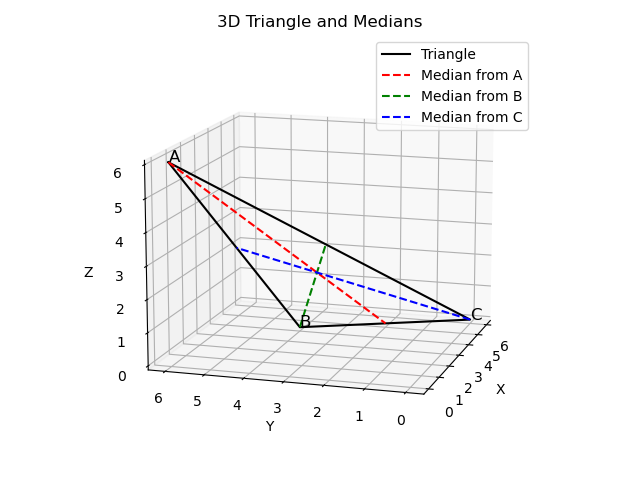
\includegraphics[width=0.75\linewidth]{./figs/Figure_1.png}
    \caption{}
    \label{fig:fig1}
\end{figure}    
\end{frame}

\begin{frame}{Conclusion}
The lengths of the medians are:


\begin{align}
\boxed{
\|\vec{AM}\| = \sqrt{61}, \quad
\|\vec{BM}\| = \sqrt{10}, \quad
\|\vec{CM}\| = 5
}
\end{align}
\end{frame}




\end{document}
